\newpage

\section{Problemi con vincoli}

CSP (Constraint satisfaction problems) è un modo di risolvere un'ampia
varietà di problemi.

In questi problemi gli stati sono definiti da \textbf{variabili $X_i$} con
valori nel dominio $D_i$.

Il \textbf{test goal} è definito da un insieme di vincoli.

La {soluzione} consiste in un insieme di valori (uno per ogni variabile) che
soddisfano tutti i vincoli.

L'idea generale è quella di eliminare larghe porzioni dallo spazio di ricerca
identificando combinazioni di valori/variabili che violano i vincoli.\\

Insieme di vincoli: $C = \{ c_i = (scope,rel_i) | i=1,...,h\}$

Lo \textbf{scope} indica le variabili interessate dal vincolo, mentre
\textbf{rel} indica quali assegnamenti di valori sono permessi.

I vincoli si classificano in:

\begin{itemize}
 \item \textbf{unari} - coinvolgono una variabile
 \item \textbf{binari} - coinvolgono una coppia di variabili
 \item \textbf{higher-order} - coinvolgono 3 o più variabili
 \item \textbf{globali} - coinvolgono un numero arbitrario di variabili
\end{itemize}

Concetti utili:

\textbf{Stato}: un assegnamento di valori a qualcuna o a tutte le variabili.

Un \textbf{Assegnamento} può essere:

\begin{itemize}
 \item \textbf{consistente} se non viola nessun vincolo
 \item \textbf{completo} se ogni variabile viene assegnata a un valore
 \item \textbf{parziale} se non è completo
\end{itemize}

Una \textbf{soluzione} è un assegnamento consistente e completo.

Un CSP binario contiene solo vincoli binari.

In un grafo di un CSP i nodi rappresentano le variabili, gli archi rappresentano
i vincoli.\\

Perché tradurre un problema in CSP? Il fatto è che molti problemi presentano
una traduzione intuitiva in un csp. Esistono sistemi generali in grado di
risolvere problemi csp senza dover costruire soluzioni su misura.
I risolutori di CSP permettono di ridurre lo spazio da esplorare grazie
alla propagazione dei vincoli.\\

Le variabili in un CSP possono essere:

\begin{itemize}
 \item \textbf{discrete}: in domini finiti di dimensione n le possibili
assegnazioni sono $\mathcal{O}(d^n)$.
 \item \textbf{continue}: coinvolgono vincoli lineari risolvibili in tempo
polinomiale (rispetto al numero di variabili) - aka programmazione lineare.
\end{itemize}

\subsection{La sottosezione degli esempi tediosi}

\textbf{Problema di soddisfacibilità booleana (3-SAT)}:\\

$(x_1 \lor x_2 \lor x_6) \land (\neg x_1 \lor x_3 \lor x_4) \land
(\neg x_4 \lor \neg x_5 \lor x_6) \land (x_2 \lor x_5 \lor \neg x_6)$

Qui ci sono 6 variabili booleane e 4 clausole (i raggruppamenti tra parentesi)
separati da $\land$.

Ogni clausola deve risultare vera affinchè tutta la formula sia
vera.

Perciò si inseriscono dei vincoli in corrispondenza di tali clausole \dots
ad esempio la tripla $(x_1, x_2, x_6)$ può assumere valori solo nel seguente
insieme: \{(0,0,1), (0,1,0), (0,1,1), (1,0,0), (1,0,1), (1,1,0), (1,1,1)\} e
così via anche per le altre (tenendo conto delle negazioni).\\

Il \textbf{problema delle n regine}: si vogliono posizionare n regine in
una scacchiera n x n in modo che con una mossa non si possano mangiare
fra di loro.\\

All'inizio si posiziona una regina su ciascuna colonna, in una riga a caso e
così facendo abbiamo escluso la possibilità di un attacco su colonna.

Occorre imporre anche altri vincoli: nessun attacco su riga e nessun attacco su
diagonale. Questi vincoli si traducono in matematichese così:

Siano $x_1,...,x_n$ le n regine posizionate su n colonne.

Sia $[1,...,n]$ la posizione su riga di una regina.

\begin{itemize}
 \item $x_i \neq x_j$: nessun attacco su riga
 \item $x_i - x_j \neq i-j$ nessun attacco su diagonale $\backslash$
 \item $x_i - x_j \neq j-i$ nessun attacco su diagonale $/$
\end{itemize}

\subsection{Formulazioni}

\textbf{Formulazione standard}:

\begin{itemize}
 \item \textbf{Stato iniziale} vuoto \{\}
 \item \textbf{Funzione successore}: assegna un valore a una delle
variabili non assegnate che non sia in conflitto con l'attuale assegnamento
 \item \textbf{Stato: assegnamento parziale}
 \item \textbf{Goal test: l'assegnamento è completo}
\end{itemize}

Con questa formulazione sarebbe possibile usare una ricerca in profondità, tuttavia
la complessità è elevata.

Se si considera un CSP con n variabili e un dominio discreto e finito di
dimensione d, viene generato un albero con $n!*d^n$ foglie anche se gli
assegnamenti completi possibili sono $d^n$\\.

In CSP, gli assegnamenti di variabili sono commutativi, perciò occorre
considerare una sola variabile a ogni nodo nell'albero di ricerca.
In questo caso il numero di foglie diventa pari al numero possibile di
assegnamenti completi, ossia $d^n$.

La ricerca in profondità in problemi CSP dove si considera l'assegnamento
di una singola variabile è chiamato \textbf{backtracking search}.

\begin{figure}[H]
\caption{Esempio di backtracking nel problema di colorazione di una mappa}
\centering
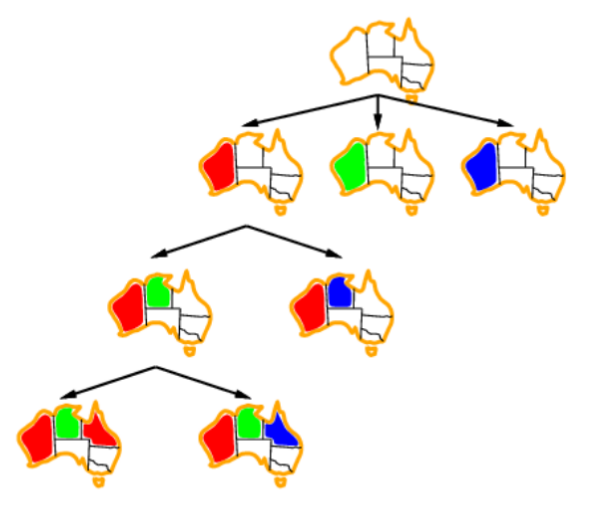
\includegraphics[width=0.5\textwidth]{backtracking}
\end{figure}

\subsection{Euristiche}

Si può scegliere di adottare l'euristica \textbf{minimum remaining values}
(MRV) che consiste nel fare branching sulla variabile a cui è possibile
assegnare il \textit{minor numero di valori}.

Un'altra euristica è la \textbf{most constraining variable} che sceglie la
variabile coinvolta nel \textit{maggior numero possibile di vincoli} con le
altre variabili.

Al contrario, l'euristica \textbf{least constraining value} sceglie la
variabile coinvolta nel \textit{minor numero possibile di vincoli} con le
altre variabili.\\

\subsection{Difetti del backtracking}


\begin{itemize}
 \item Non ricorda le ragioni di eventuali conflitti; la soluzione è il
\textbf{backjumping}.
Il \textbf{backjumping} consiste nel ritornare all'assegnamento completo causa del
conflitto e identificare la più recente assegnazione precedente.

 \item Effettua più volte controlli inutili; la soluzione è \textbf{ricordarsi gli
assegnamenti non legali} e aggiungere dei vincoli al problema o tenere in cache
tali assegnamenti e controllare che non vengano ripetuti.

 \item Un conflitto viene scoperto solo quando tutte le variabili sono state assegnate a
dei valori; la soluzione è fare \textbf{forward checking} dei vincoli (si controlla
in anticipo se un assegnamento non completo porterà alla violazione di un vincolo).
Come? Tenendo in considerazione i valori legali delle rimanenti variabili. Quando a
una certa variabile non ancora assegnata non rimangono più valori legali, si scopre
in anticipo il conflitto (si veda la figura \ref{fig:fc})\dots ma non prevede
altri tipi di possibili conflitti (ad esempio quando due variabili rimanenti possono
assumere lo stesso unico valore).
\end{itemize}

\begin{figure}[H]
\centering
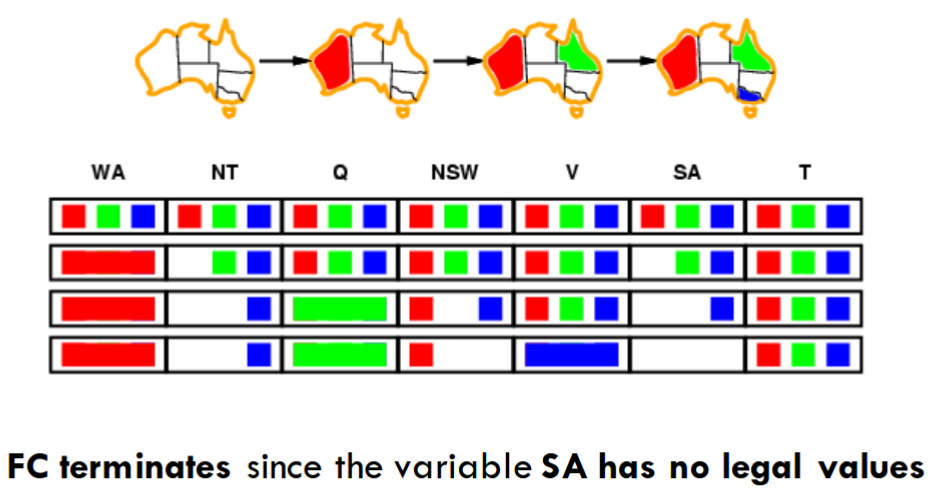
\includegraphics[width=0.5\textwidth]{fc}
\caption{Esempio di forward checking nel problema di colorazione di una mappa}
\label{fig:fc}
\end{figure}

Per risolvere la previsione dei conflitti e migliorare il forward checking viene
usata la \textbf{propagazione dei vincoli}, al fine di assicurare la
consistenza locale del problema. Esistono diversi tipi di consistenza\dots

\begin{itemize}
 \item \textbf{Nodo-consistenza}: una variabile è nodo consistente se tutti
i valori nel suo dominio soddisfano i vincoli unari imposti.
 \item \textbf{Arco-consistenza}: una variabile è arco consistente se tutti
i valori nel suo dominio soddisfano i vincoli binari imposti.
Assumiamo che ci sia un vincolo binario tra X e Y: X è arco consistente
rispetto a Y se e solo se per ogni valore di X, esiste un valore \textbf{legale}
di Y:\\

X arco consistente con Y $\iff (\forall$ valore di X $\implies \exists$ valore
legale di Y)\\

Ne segue che ogni volta che il dominio di X viene ristretto di un valore,
occorre ricontrollare tutti i suoi vicini per assicurare ancora l'arco consistenza.
L'arco consistenza rileva un fallimento \textbf{prima del forward checking}.

In generale verificare che un problema csp sia AC permette di restringere lo spazio
delle soluzioni, ma non può dirci con certezza se esiste una soluzione (e
restituirne una - quando tutti i domini delle variabili sono ristretti a un unico
valore) o se non ne esiste nessuna (quando rimangono domini vuoti per una o più variabili).
 \item \textbf{Cammino-consistenza}: si tratta di imporre la consistenza su più di un
vincolo. Due variabili legate da un vincolo ${X_i, X_j}$ sono cammino-consistenti rispetto
a una terza variabile $X_m$ se per ogni assegnamento consistente di
${X_i, X_j}$ esiste un assegnamento di $X_m$ che soddisfa i vincoli di ${X_i, X_m}$
e ${X_i, X_j}$.
\end{itemize}

Un concetto più generale di consistenza è la k-Consistenza\dots un problema
CSP è k-consistente se per ogni insieme di k-1 variabili e per ogni assegnamento
consistente di queste k-1 variabili, può sempre essere scelto un valore consistente
per una qualsiasi variabile k-esima.

\begin{itemize}
 \item Nodo consistenza $\rightarrow$ 1-consistenza
 \item Arco consistenza $\rightarrow$ 2-consistenza
 \item Cammino consistenza $\rightarrow$ 3-consistenza
\end{itemize}

\subsection{Local search}

Nell'ambito dei problemi con vincoli è possibile applicare la ricerca
locale come segue:

Lo scopo è quello di ``migliorare'' un assegnamento di variabili, cercando di
diminuire man mano il numero di vincoli violati.

Lo spazio di ricerca in questo problema sono tutti gli assegnamenti completi.

Il vicinato di un assegnamento sono tutti gli assegnamenti che possono essere
raggiunti tramite un passo della ricerca locale, cioè tutti gli assegnamenti
che differiscono per il valore di una variabile.

Lo spazio delle soluzioni invece consiste di tutti gli assegnamenti che
soddisfano i vincoli.

La funzione di valutazione mappa gli assegnamenti a un numero reale che indica
quanto sono lontani dall'essere una soluzione, cioè il numero di vincoli
violati.

La ricerca comincia da un assegnamento casuale e si muove verso i suoi vicini
in base alla funzione di valutazione. Termina quando trova una soluzione o
ha effettuato un certo limite di passi.

Una possibile euristica che utilizza la funzione di valutazione e guida la
ricerca locale è la \textbf{Min-Conflicts}. Questa euristica scegli il vicino
di un assegnamento che minimizza il numero di conflitti violati.

\begin{algorithm}
    \caption{Euristica Min-Conflicts}
    \label{alg:minconflicts}
    \begin{algorithmic}[1]
        \Procedure{MIN-CONFLICTS}{csp, max\_steps}
            \State{current $\leftarrow$ un assegnamento completo per csp}
            \For{i = 1 to max\_steps}
            \If{current è una soluzione per csp} \Return{current} \EndIf
            \State{var $\leftarrow$ una qualsiasi variabile coinvolta in un
conflitto}
            \State{value $\leftarrow$ un valore per var che minimizzi i
conflitti dell'assegnamento current}
            \State{var = value in current}
            \EndFor
            \State{\Return{Fallimento}}
        \EndProcedure
    \end{algorithmic}
\end{algorithm}

Anche se nell'ambito dei problemi con vincoli, il principio della ricerca
locale è sempre lo stesso e anche i problemi rimangono gli stessi:
è possibile bloccarsi in un minimo locale (largo o stretto) o in un plateau.

Tecniche per evitare di bloccarsi:

\begin{itemize}
 \item Ricominciare da stati iniziali casuali
 \item Permettere passi non miglioranti $\rightarrow$ random-walk
 \item Cambiare il vicinato $\rightarrow$ taboo search
 \item Cambiare la funzione di valutazione $\rightarrow$ strategie penalty-
based
\end{itemize}

Rimanere intrappolati in un minimo locale può essere visto come bloccarsi
in un loop. Per sbloccarsi da un loop si possono ricordare gli stati
già visti e non visitarli più: questo potrebbe consumare molta memoria,
perciò è utile memorizzare solo gli ultimi stati per prevenire ``piccoli''
loops.

La lista tabù contiene gli stati vietati <variabile, valore> e ha una lunghezza
fissata k.

